\subsection{GTKWave data flow}
\label{sec:GTKWaveDataflow}

A way to debug and follow the data flow in the CPU, is to analyze it in GTKWave\footnote{\url{http://gtkwave.sourceforge.net}} as seen in figure \ref{fig:GTKWave}. 

\begin{figure}[H]
    \centering
    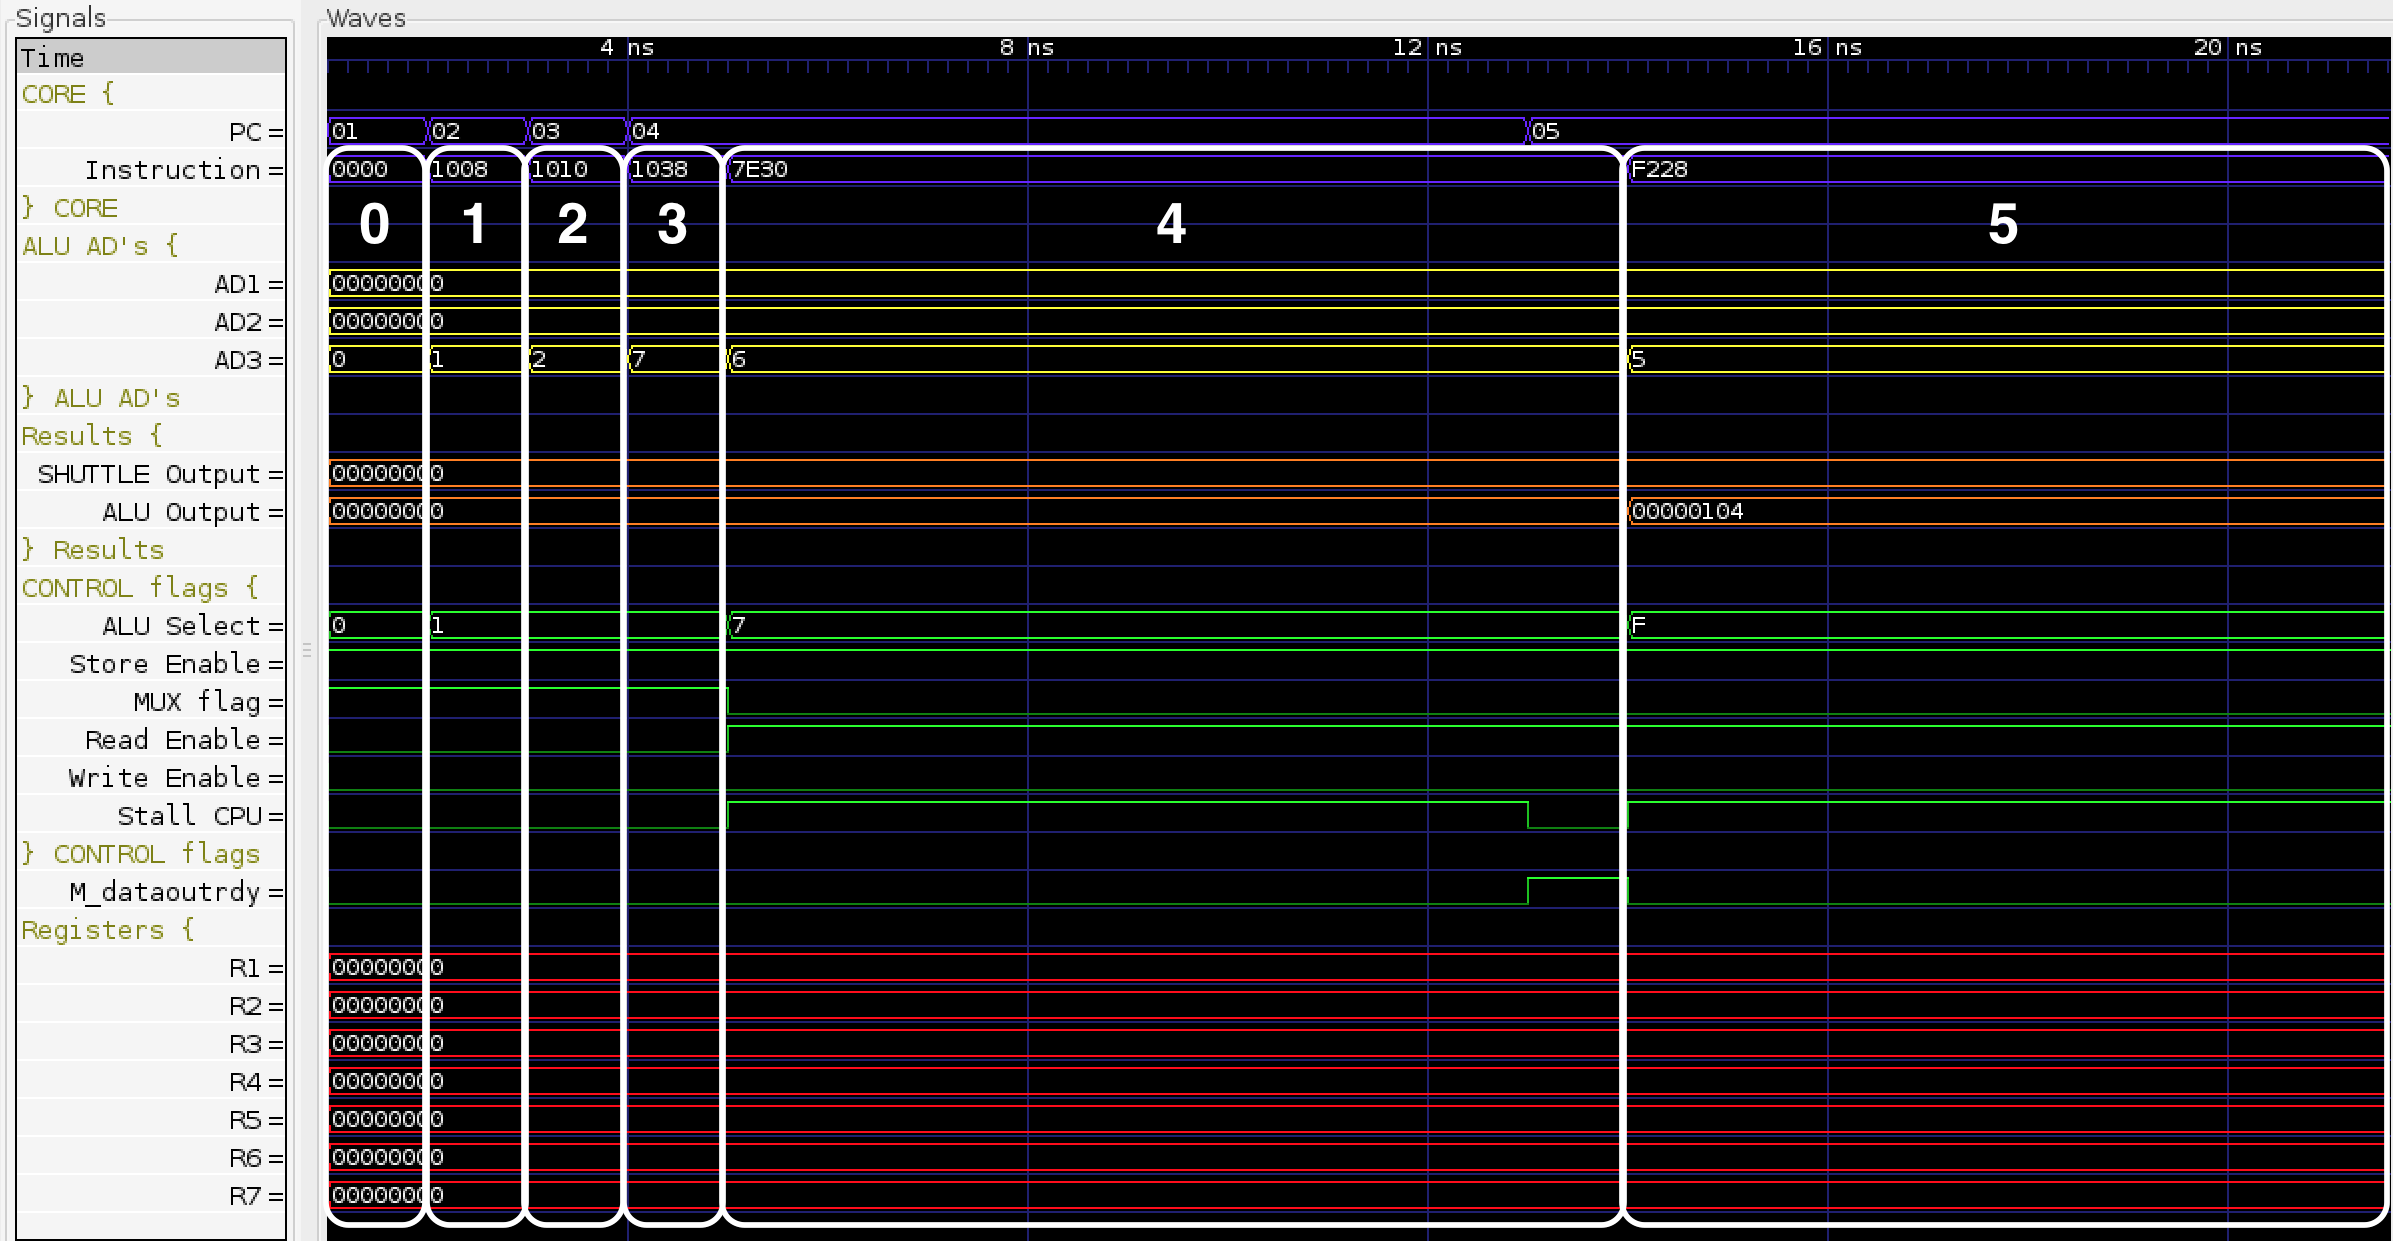
\includegraphics[width=\textwidth]{3Results/fig/GTKWave.png}
    \caption{Analyzing the CPU data flow in GTKwave in the initial state. Appendix \ref{app:GTKWave} has a large print-friendly version.}
    \label{fig:GTKWave}
\end{figure}

As seen on figure \ref{fig:GTKWave}, we have split the figure into segments 0 through 5, corresponding to the first five instructions in our program instructions (see table \ref{table:ProgInstructionSet}). These sections refer to the initialization state and the first step of the algorithm (see section \ref{sec:AlgIns}).\\

\textbf{Segment 0:} \\
This section is the consequence of the used \texttt{ipblock}. Since the \texttt{ipblock} is one cycle behind, the first instruction (line 0) of the program instruction set is equal to a \texttt{NOP}. When the \texttt{ipblock} reads a \texttt{NOP} (or an empty line), it is treated as a line 0's.
The ipblock continues to be one cycle behind, so the the values set in e.g. segment 1 are set when PC=1. (Hence the numbering in figure \ref{fig:GTKWave})\\

\textbf{Segment 1:} \\
The CPU has now received the first instruction, which is to set R1's value\footnote{For the general use of registers in this program setup, see segment \ref{sec:registers}.}  to the value from R0. While this is happening, all other components are in an idle state, since everything works in parallel. The \texttt{ALU\_select} is set to 1 from \texttt{CONTROL}, telling the \texttt{ALU} to simply forward the value from R0 (since AD1 = 0). \\

\textbf{Segments 2 and 3:} \\
Instructions 2 and 3 resemble instruction 1. Since this is in the initialization state of the CPU, in which we make sure that certain registers contain the value 0 when the calculations start. The values are stored in R2 and R7. Since we store the values 0, and the registers already contain the values 0, it is difficult to see this step in GTKWave waveforms. \\

\textbf{Segment 4:} \\
Instruction 4 is \texttt{LOAD}, loading the new data value from the data list in memory from address R7 and storing the value in R6. Since the value is loaded from memory, the CPU is set to \texttt{stall} while waiting for the \texttt{BUS} to return with the required value. The way the CPU is set to \texttt{stall} is by preventing the \texttt{PC} from incrementing. This results in the CPU keep trying to load from memory, storing trash values in the register specified by \texttt{AD3} until the correct value is received. In order to synchronize this process, the \texttt{stall} signal (called \texttt{Stall CPU} in figure \ref{fig:GTKWave}) is set true if either \texttt{Read Enable} or \texttt{Write Enable} is true. Once the \texttt{M\_dataoutrdy}\footnote{Preimplemented signal from \texttt{BUS} template.} signal is true (telling the CPU that the \texttt{BUS} has returned from memory), \texttt{Stall CPU} is set to false. This ensures that the last value collected from \texttt{SHUTTLE} is the correct value. \\
The value returned from \texttt{BUS} through \texttt{SHUTTLE} in this case is 0, since this is the data at line 0 in the data list. \\

\textbf{Segment 5:} \\
Instruction 5 is \texttt{LOADC}, loading the old data point from the circular array in memory from address R1 (shifted through the \texttt{ALU}), storing the value in R5. The loading process is the same as described in segment 4. \\
The value returned through this load procedure is also 0, since it loads from the circular array which is initialized to 0's by default. The interesting part in this segment is the \texttt{ALU Output} value which changes from 0 to 0x104. Since the command is \texttt{LOADC}, the address is shifted 260 places through the \texttt{ALU}. 0x104 in hex = 260 in decimal.